%!TEX root = ../thesis.tex
%*******************************************************************************
%****************************** Second Chapter *********************************
%*******************************************************************************

\chapter{On the quantum many-body problem}
\label{chapter2}
This chapter discusses the quantum many-body problem and numerical approaches to its solution. We begin by introducing the Schr\" odinger equation and Feynman path integral formulations of quantum mechanics, before briefly discussing lattice models and their significance. We then turn our attention towards solution procedures, providing a primer on popular methods with an emphasis on stochastic, Monte Carlo, approaches. Finally, we highlight recent usage of machine learning methods in this field.

\ifpdf
    \graphicspath{{Chapter2/Figs/Raster/}{Chapter2/Figs/PDF/}{Chapter2/Figs/}}
\else
    \graphicspath{{Chapter2/Figs/Vector/}{Chapter2/Figs/}}
\fi

%********************************** %First Section  **************************************
\section{The Schr{\"o}dinger equation and the Feynman path integral}
\label{subsec:latt-qm}
The dynamics of a quantum mechanical system are described with the Schr\" odinger equation
\begin{equation}
\label{eq:sch}
i \hslash \frac{\mathrm{d}}{\mathrm{d} t}|\Psi(t)\rangle=\hat{H}|\Psi(t)\rangle,
\end{equation}
a linear partial differential equation. The state of the quantum system $| \Psi \rangle$ is a vector in a separable Hilbert space $\mathcal{H}$, and the square of its absolute value, e.g. $|\Psi(x, t)|^2$, at each point is interpreted as a probability density function (pdf). The Hamiltonian operator is the sum of kinetic and potential energies $\hat H = \hat T + \hat V$ of the system. Throughout this thesis we will be interested only in the ground state of the system, this is the state with lowest energy and it is the state we find the system in at zero-temperature. Instead of using the time-dependent formulation in eq.~\eqref{eq:sch}, we use the \emph{stationary} Schr\" odinger equation
\begin{equation}
\hat{\mathrm{H}}|\Psi\rangle=E|\Psi\rangle,
\end{equation}
an eigenvalue equation, with the lowest energy $E_0$ corresponding to the ground state $|\Psi_{0}\rangle$. From this point onward, we use Hartree atomic units $m_{e}=e=\hslash=a_{0}=\mathrm{E}_{h}=k_{e}=1$.

Alternatively to the Schr\" odinger equation one can use an integral Green's function representation to express the wavefunction $\Psi$ at some future time $t$ given initial condition $\Psi(x^\prime, t^\prime)$ as
\begin{equation}
\Psi\left(x, t\right)=\int  \mathcal{K}\left(x, t ; x^\prime, t^\prime\right) \Psi\left(x^\prime, t^\prime\right) \mathrm{d} x^\prime.
\end{equation}
The \emph{propagator} $\mathcal{K}\left(x, t ; x^\prime, t^\prime\right)$ is the kernel of the Schr\" odinger equation
\begin{equation}
\left(i \frac{\partial}{\partial t}-H_{x}\right) \mathcal{K}\left(x, t ; x^\prime, t^\prime\right)=i \delta\left(x - x^\prime\right) \delta\left(t-t^\prime\right).
\end{equation}
It is related to the fundamental solution or Green's function as
\begin{equation}
\mathcal G\left(x, t ; x^{\prime}, t^{\prime}\right)=\frac{1}{i} \Theta\left(t-t^{\prime}\right) \mathcal K\left(x, t ; x^{\prime}, t^{\prime}\right),
\end{equation}
where $\Theta$ is the Heaviside function and $\delta$ is the Dirac delta. The same propagator can also be expressed using the Feynman path integral
\begin{equation}
\label{eq:FPI}
\mathcal{K}\left(x, t ; x^\prime, t^\prime\right)=\int_{\substack{q(t)=x \\ q(t^\prime)=x^\prime}} \exp \left(i \int_{t^\prime}^{t} \mathcal{L}(q, \dot{q}, t) d t\right)\mathcal{D}[q(t)],
\end{equation}
where $\mathcal{L}$ is the classical Lagrangian function of the system, and the path integral is over all paths that satisfy the endpoint conditions $q(t)=x, q(t^\prime)=x^\prime$. This formulation of QM is closely related to the approaches we will develop in the later chapters. 

\section{Lattice models}
\label{sec:lattice-models}
Lattice quantum spin systems, or lattice models for short, play a very important role in the modern condensed matter physics landscape. They are idealisations of real world systems that are conceptually simple, but still exhibit very rich physics. Take the physics of cuprate superconductors as an example, cuprates are composed of layers of copper oxides alternating with layers of other metal oxides and by neglecting intra-layer coupling the physics of the magnetic excitations can be considered mostly two dimensional. The study of lattice systems in one and two dimensions has been especially productive, 
as many exact solutions containing non-trivial physics have been found. Concretely, spin systems that exhibit phase transitions provide insight into thermal and quantum fluctuations driving the such transitions~\cite{parkinson2010introduction}.

\subsection{Examples of lattice models}
\label{subsec:latt-examples}
Lattice models have long been used to study magnetism, and perhaps the most famous model is the Heisenberg model~\cite{heisenberg1985theorie},
\begin{equation}
\label{eq:general_heisenberg}
\hat H = -\sum_{ij} \sum_{\alpha\beta} J^{\alpha \beta}_{ij} S^{\alpha}_{i} S^{\beta}_{j} + \sum \vec{B}\cdot \vec{S}_i,
\end{equation}
where $\vec{B}$ is the external magnetic field, $i, j$ are lattice sites, and the spin-spin interaction between spin-vector components $\alpha, \beta \in \{x, y, z\}$ at sites $i, j$ is given by $J^{\alpha \beta}_{ij}$. The general problem in eq.~\eqref{eq:general_heisenberg} cannot be solved, but some special cases in low dimensions have analytical solutions. One such case is the \textbf{transverse field Ising model} (TFIM)~\cite{de1963collective}, which is obtained by setting
\begin{equation}
	J^{\alpha \beta}_{ij} = J \delta_{\langle i, j \rangle} \delta_{\alpha, \beta} \delta_{\alpha, z}, \quad \vec{B} = -B \vec{e}_x, \quad \text{ and } \quad S = \frac{1}{2},
\end{equation}
thus
\begin{equation}
	\label{eq:h-ising}
	\hat H_{\mathrm{Ising}}=-J \sum_{\langle i, j\rangle} \hat{\sigma}^z_{i} \hat{\sigma}^z_{j}-h \sum_{i} \sigma^x_{i},
\end{equation}
where $\langle i, j\rangle$ denotes a sum over nearest neighbours. A spin-$\frac{1}{2}$ system is represented in terms of Pauli matrices $\hat \sigma_i^{\alpha}$ acting on spin at site $i$
\begin{equation}
\hat{\sigma}^x_{i}=\left(\begin{array}{cc}0 & 1 \\ 1 & 0\end{array}\right)_{i} \quad \hat{\sigma}^y_{i}=\left(\begin{array}{cc}0 & -i \\ i & 0\end{array}\right)_{i} \quad \hat{\sigma}^z_{i}=\left(\begin{array}{cc}1 & 0 \\ 0 & -1\end{array}\right)_{i}.
\end{equation}
The Hilbert space of a single spin is two-dimensional, we construct its basis in terms of $\hat \sigma^z$ eigenvalues $\{|\uparrow\rangle,|\downarrow\rangle\}$, where $\hat{\sigma}^{z}|\uparrow\rangle=|\uparrow\rangle \text { and } \hat{\sigma}^{z}|\downarrow\rangle=-|\downarrow\rangle$. Pauli matrices at different sites commute
\begin{equation}
	\left[\hat{\sigma}_{i}^{\alpha}, \hat{\sigma}_{i^{\prime}}^{\alpha^{\prime}}\right]=0 \quad \text { for } \quad i^{\prime} \neq i, 
\end{equation}
and follow 
\begin{equation}
	\left[\hat \sigma^\alpha_{i}, \hat \sigma^\alpha_{k}\right]=2 i \varepsilon_{j k \ell} \hat \sigma^\alpha_{\ell}
\end{equation}
on the same site $i$. We define raising and lowering operators $\hat{\sigma}_{i}^{\pm}$ as
\begin{equation}
\hat{\sigma}_{i}^{\pm} = \left(\hat{\sigma}_{i}^{x} \pm i \hat{\sigma}_{i}^{y}\right) / 2, \quad \text{where} \quad \hat{\sigma}^{+}|\downarrow\rangle=|\uparrow\rangle \text { and } \hat{\sigma}^{-}|\uparrow\rangle=|\downarrow\rangle.
\end{equation}
The whole Hamiltonian then acts on the tensor product space $\left(\mathbb{C}^{2}\right)^{\otimes N}$ with dimension $2^N$. The TFIM has been exhaustively studied~\cite{stinchcombe1973isingI, stinchcombe1973isingII}, one-dimensional case was solved by Pfeuty~\cite{pfeuty1970one}, the solution uses Jordan-Wigner transformation of spin operators to spinless fermions~\cite{lieb1961two, niemeijer1967some}. The one dimensional case has two distinct states, the ordered phase for $|h| < J$ is either ferromagnetically $J > 0$ or anti-ferromagnetically $J < 0$ ordered. Since this state breaks spin-flip symmetry it is doubly degenerate, for $h=0$ and $J>0$ we have either $|\uparrow \uparrow \cdots \uparrow \rangle$ or $|\downarrow \downarrow \cdots \downarrow \rangle$. The system undergoes a quantum state transition at $|h| = J$ into a disordered phase for $|h| > J$, for $h \rightarrow \infty$ we have either $|\rightarrow \rightarrow \cdots \rightarrow \rangle$. 


The \textbf{XY model}~\cite{lieb1961two} is another spin model that can be solved using the Jordan-Wigner transformation, its Hamiltonian is
\begin{equation}
	\label{eq:h-xy}
\hat H_{\text{XY}}=-\frac{1}{2} \sum_{\langle i, j\rangle} \hat\sigma_{i}^{x} \hat\sigma_{j}^{x}+\hat\sigma_{i}^{y} \hat\sigma_{j}^{y}.
\end{equation}
More generally, we can write a Hamiltonian for a chain of spins by setting $J_{i j}^{\alpha \beta} = J_\alpha \delta_{\alpha \beta} \delta_{i, j+1}$ and $\vec{B} = -h \vec{e}_z$
\begin{equation}
	\label{eq:h-xyz}
	\hat H_{\text{XYZ}}= -\frac{1}{2}\left[ \sum_{j=1}^{N}J_{x} \hat \sigma_{j}^{x} \hat \sigma_{j+1}^{x}+J_{y} \hat \sigma_{j}^{y} \hat \sigma_{j+1}^{y}+J_{z} \hat \sigma_{j}^{z} \hat \sigma_{j+1}^{z} + h \sigma_{j}^{z}
	\right],
\end{equation}
this is the \textbf{XYZ Heisenberg chain}. It is another well studied model with solutions for various settings of the coupling constants $J_\alpha$. The isotropic ferromagnetic XXX chain ($J_x = J_y = J_z = J < 0$) was solved by Bethe with his famous ansatz~\cite{bethe1931theorie}. The ground state~\cite{hulthen1938austauschproblem} and excitations~\cite{des1962spin} of the isotropic antiferromagnetic XXX chain ($J_x = J_y = J_z = J < 0$) are known, and so are the solutions to the XXZ chain ($J_x = J_y = J \neq J_z$)~\cite{yang1966three, yang1966one, yang1966two} and the fully anisotropic XYZ chain ($J_x \neq J_y \neq J_z$)~\cite{baxter1972one}. 

Models discussed so far only include nearest-neighbour interactions, a model which includes next nearest-neighbour interactions is the $\mathbf{J1}$\textbf{-}$\mathbf{J2}$ \textbf{model}
\begin{equation}
	\label{eq:h-j1j2}
	\hat H_{J_1\text{-}J_2} = J_1 \sum_{\langle i, j \rangle} \mathbf{\hat \sigma}_i \mathbf{\hat \sigma}_j + J_2 \sum_{\langle\langle i, j \rangle\rangle} \mathbf{\hat \sigma}_i \mathbf{\hat \sigma}_j.
\end{equation}
We now turn our attention to general approaches to the quantum many body problem, we will return to models again when discussing stoquastic Hamiltonians in sections~\ref{subsec:fk-latt} and~\ref{sec:stoq_latt_forms}.

\section{Approaches to the quantum many-body problem}
\label{sec:QMBP}
The quantum many-body problem, which amounts to solving the $3N$-dimensional Schr\"odinger equation, underpins a large part of quantum chemistry, condensed matter physics and materials science. The problem is notoriously hard to solve and very few systems with analytical solutions exist, most of them constrained in some artificial way such that they lend themselves to mathematical analysis. Along with spin models mentioned before, examples include the Hookium atom, an analogue of helium where two electrons interact with the nucleus via a Hookean potential, and Spherium, a system of two electrons confined to the surface of a sphere. Great efforts have been made in the nearly 100 years since the conception of the Schr\" odinger equation, in developing both analytical and numerical techniques to produce insights into quantum systems. Perhaps the most impactful was the development of various approximate methods that solve the many-body problem with our limited computational resources. While there is ongoing work on quantum simulators and computers that could greatly speed-up solving quantum problems~\cite{feynman2018simulating, childs2010relationship}, we here discuss methods one can use with a classical computer. The commonality of all mentioned methods is that they try to tame the exponential growth of the underlying Hilbert space w.r.t the system size, they differ in how they achieve this. The three most common assumptions/simplifications to the many-body problem employed in condensed matter and quantum chemistry are the Born-Oppenheimer approximation, that electronic motion is instantaneous compared to the nuclear motion, the use of chemical basis sets, which transforms the PDE into an algebraic problem, and usually neglecting relativistic effects.

\subsubsection{Hartree-Fock}
One of the most common approaches to the many-body problem is to replace the original interacting many-body problem with a set of independent-particle problems with effective potential. \textbf{Hartree-Fock} (HF) approaches solve an auxiliary system of independent electrons in a self-consistent field and assume that the wave function (for fermions) can be represented as a single Slater determinant. The HF method does not include electron correlation, which makes it a good approximation only in systems where correlation contributions are small. 

\subsubsection{Post-Hartree-Fock methods}
Post-HF methods, such as Coupled Cluster, Configuration interaction and M\o ller-Plesset theory include correlation by considering a linear combination of Slater determinants. They can be extremely accurate but come at a high computational cost. 

\subsubsection{Density Funcitonal Theory}
Alternatively \textbf{Density Functional Theory} (DFT) reformulates the many-body electron problem in terms of the $3$-dimensional electron density $n(\mathbf{r})$, which is found by minimising the total energy functional $E[n(\mathbf{r})]$~\cite{hohenberg1964inhomogeneous}. In practice this is done by solving the Kohn-Sham auxiliary system. DFT is in theory exact, however only if the true energy functional $E[n(\mathbf{r})]$ is known. As this is not the case, much research has been done in constructing different energy functionals with varying degrees of accuracy, starting with local functionals e.g. LSDA and continuing towards more heavily parameterised, non-local formulations. DFT provides a good trade-off between accuracy and computation time, it is used extensively for simulating large systems as linear scaling variants of DFT exist~\cite{skylaris2005introducing}. 

\subsubsection{Dynamical Mean Field Theory}
DMFT~\cite{held2007electronic} is a framework that is specialised in solving strongly correlated systems. It is intuitively similar to Weiss Mean Field Theory in classical statistical physics. The main idea is to map an intractable lattice problem into an impurity model in an effective medium, a many-body local problem which can be solved with any standard approach (QMC, DFT, exact diagonalisation, etc.). This mapping between lattice and impurity model is exact, the approximation comes in neglecting spatial fluctuations of the lattice self-energy $\Sigma$, the contribution to energy due to particle interaction with medium. DMFT assumes that $\Sigma$ is a function of frequency and not momentum $\Sigma(k, \omega) = \Sigma(\omega)$, which only holds in the infinite coordination case. Time fluctuations are taken into account, i.e. the effective medium is not static in DMFT, which is an advantage over other static mean field theories. 

\subsubsection{Density Matrix Renormalization group}
DMRG~\cite{white1992density} is considered the state of the art method for solving one-dimensional lattice problems, it has been widely adopted in condensed matter physics, first used to solve the system of a spin-0 particle in a box. It is an iterative method based on the renormalization group~\cite{wilson1975renormalization}, and uses matrix product states as the variational ansatz. The method has also been extended for time evolution of systems~\cite{feiguin2005time}, and higher dimensions~\cite{verstraete2004renormalization}.

\subsection{Stochastic methods - Quantum Monte Carlo}
\label{subsec:qmc-overview}
%% General about QMC
Quantum Monte Carlo is a class of methods that uses statistical sampling to directly deal with high-dimensional integration that arises from working with the many-body wave function. QMC methods are among the most accurate achieving chemical accuracy for smaller systems~\cite{foulkes2001quantum}, and can in principle achieve any degree of statistical precision sought. A large ecosystem of QMC methods exists, and they have been adapted to study almost any quantum system imaginable, from discrete to continuous state space, fermionic and bosonic systems, as well as both finite and zero temperatures. Even though QMC methods are not computationally the cheapest, they have reasonable storage requirements as the wave function does not need to be stored directly. Moreover, the high computational cost of QMC methods can be aided by paralellisation and use of hardware acceleration, as the core calculation in is repetitive and usually involves generating (pseudo)-random numbers, performing a simple calculation and in the end averaging over the results. 

%% Zero temperature methods
%% Variational quantum monte carlo
\subsubsection{Variational quantum Monte Carlo (VMC)}
The most straightforward QMC approach is based on the variational principle, which provides a clear path towards a solution to the ground state problem. Simply use a \emph{trial wave function} $\Psi_{T}$ to parameterise the ground state and optimise the parameters of $\Psi_{T}$ to reach the lowest-energy state. This lowest variational state should capture the behaviour of the ground state if the ansatz is expressive enough. The flexibility of easily defining the trial wave function for a variety of different problems and the ease of its evaluation is a clear advantage over methods described in the previous section. Moreover, given that the variational wave function should encapsulate the main aspects of the system studied it provides intuition into the system itself. Development of trial functions has played a key role in the applicability of VMC, famous examples of trial wave functions include the Slater-Jastrow and Backflow wave functions. The drawback of VMC is that the variational wave function might contain a bias that cannot be avoided through optimisation of the parameters alone, see Fig.~\ref{fig:qmc_blocking}. 
\begin{figure}[h]
	\centering
	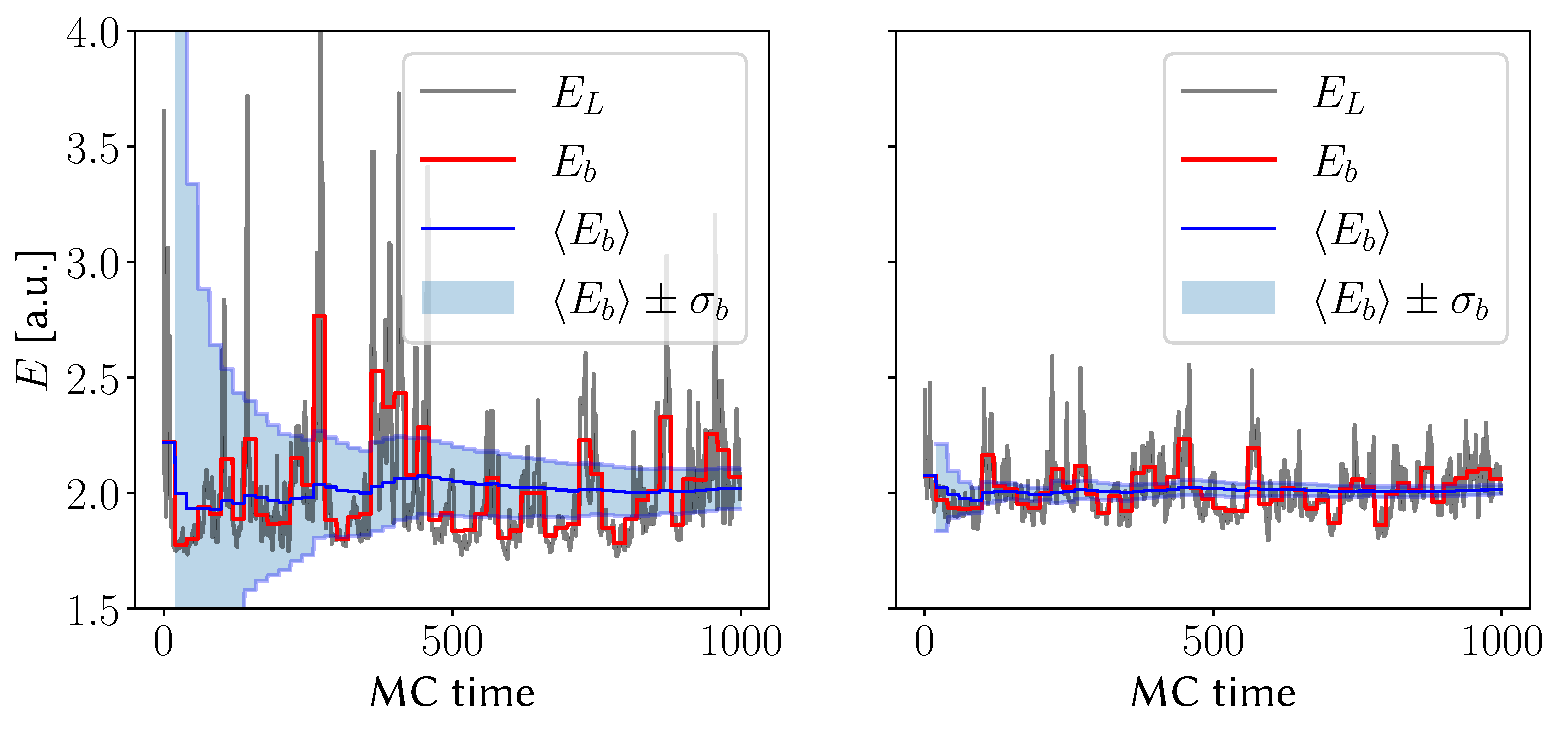
\includegraphics[width=\linewidth]{Chapter2/Figs/Vector/blocking}
	\caption[Ansatz quality in VMC]{\textbf{Ansatz quality in VMC}. Appropriateness of the variational wave function limits the quality of VMC, a poor choice of ansatz results in typical spikes in local energy  and biased result (\textbf{left}), as well as slower convergence than a good trial wave function (\textbf{right}). Figures show the local energy $E_L$, reblocked average energy $\langle E_b \rangle$ and variance $\sigma_b$ of a VMC simulation of Hookium.}
	\label{fig:qmc_blocking}
\end{figure}
VMC necessarily contains two steps, first is the estimation of the variational energy and second is the optimisation of the parameters. Any expectation of an operator $\hat{O}$ can be expressed in terms of the trial wave function as
\begin{equation}
	\langle\hat{O}\rangle=\frac{\langle\Psi_{T}\mid\hat{O}\mid \Psi_{T}\rangle}{\langle\Psi_{T} \mid \Psi_{T}\rangle}=\frac{\sum_{x}\langle\Psi_{T} \mid x\rangle\langle x\mid\hat{O}\mid \Psi_{T}\rangle}{\sum_{x}\langle\Psi_{T} \mid x\rangle\langle x \mid \Psi_{T}\rangle},
\end{equation}
where $\mid x \rangle$ are orthogonal and normal states of the Hilbert space. If we rewrite the above expression as 
\begin{equation}
	\label{eq:vmc-local_op_sampling}
	\langle \hat{O} \rangle = \frac{\sum_{x}\mid\Psi_{T}(x)\mid^{2} \hat{O}_{L}(x)}{\sum_{x}\mid\Psi_{T}(x)\mid^{2}},
\end{equation}
with $\hat{O}_L$ being the \emph{local operator}
\begin{equation}
	\hat{O}_{L}(x)=\frac{\langle x\mid\hat{O}\mid \Psi_{T}\rangle}{\langle x \mid \Psi_{T}\rangle}, 
\end{equation}
	we can interpret $|\Psi(x)|^{2}/\sum_{x}|\Psi(x)|^{2}$ as a probability. Meaning that eq.~\eqref{eq:vmc-local_op_sampling} can be estimated as an average of the local operator $\hat{O}_L$
\begin{equation}
	\langle\hat{O}\rangle \approx \frac{1}{M} \sum_{m=1}^{M} \hat{O}_{L}\left(x_{m}\right),
\end{equation}
sampled from this probability distribution. The sampling can be done using Markov Chain Monte Carlo (MCMC). The second step of the procedure is variational optimisation of the trial wave function, where the optimal parameters of the approximation are found by minimising the \emph{cost function}. The straightforward choice of the variational energy $E_V$ as a cost function turns out to be inferior to minimizing the \emph{variance} of the energy $\sigma_E$~\cite{foulkes2001quantum}. This is because $\sigma_E$ obeys the \emph{zero-variance} property, meaning that if $\Psi_{T}$ is an exact eigenvalue of the Hamiltonian
\begin{equation}
	\hat{H}\left|\Psi_{T}\right\rangle=E_{V}\left|\Psi_{T}\right\rangle,
\end{equation}
then the local energy $E_L$ is constant and equal to $E_V$
\begin{equation}
	E_{L}(x)=\Psi_{T}(x)^{-1} \hat{H} \Psi_{T}(x)=\Psi_{T}(x)^{-1} E_{V} \Psi_{T}(x)=E_{V},
\end{equation}
irrespective of the sampled configuration $x$ and hence has zero variance. The zero-variance property has important consequences for numerical stability of optimisation, it means that energy variance minima are robust to finite sampling. Minimizing the variance of energy drives the trial wave function towards eigenstates of the Hamiltonian. Moreover, the statistical error of any expectation value $\langle \hat{O} \rangle$ is proportional to the variance of $\hat{O}$, making low variance doubly desirable. There are several approaches to updating the parameters each iteration, gradient descent, stochastic reconfiguration~\cite{sorella1998green}, and the linear method~\cite{nightingale2001optimization} are just a few examples. It is crucial that the methods are robust to statistical noise and converge quickly as the MC step can be expensive to perform. Moreover they are only as good as the estimates of the energy (variance) gradients w.r.t the parameters.

The first application of VMC was to the ground state ${}^4$He~\cite{mcmillan1965ground} and it was later extended for studying many-body fermionic systems~\cite{ceperley1977monte}. Time-dependant variants of this method exist~\cite{becca2017quantum} and VMC has been used to study non-equilibrium properties of bosonic~\cite{carleo2012localization, carleo2014light}, and fermionic~\cite{ido2015time} systems.

%% Green function QMC and Diffusion QMC
\subsubsection{Projector QMC (PMC) techniques}
\label{subsubsec-PMC}
PMC is a class of QMC methods which are in essence nothing more than stochastic implementations of the power method to obtain the dominant eigenvector of a matrix or a kernel function~\cite{gubernatis_kawashima_werner_2016}. Their distinct advantage over VMC is that they are not constrained by our parametrisation of the trial wave function, as they can describe arbitrary probability distributions. PMC methods are based on the imaginary Schr\" odinger equation
\begin{equation}
	\label{eq:imgsch}
	\partial_{t}\left|\Psi_{t}\right\rangle=-\hat{H}\left|\Psi_{t}\right\rangle.
\end{equation}
Its formal solution, the time propagation of an initial wave function $|\Psi_0\rangle$ at $t=0$, is written as
\begin{equation}
\left| \Psi_{t} \right\rangle = e^{-\hat{H} t}\left|\Psi_{0}\right\rangle. 
\end{equation}
From the spectral decomposition of the operator $e^{-\hat{H} t}$ in terms of eigenstates $|\Phi_n\rangle$ and eigen-energies $E_n$ of the Hamiltonian $\hat{H}$
\begin{equation}
\label{eq:spectral_decompH}
e^{-\hat{H} t}=\sum_{n} e^{-E_{n} t}|\Phi_n\rangle\langle\Phi_n|, 
\end{equation}
it follows that the term corresponding to the ground state of the system $|\Phi_0\rangle$ decays the slowest. Thus starting in some initial state and propagating for a long imaginary time $it$ leads into the ground state with the decay rate giving the ground state energy $E_0$ as
\begin{equation}
\label{eq:long_time_limit_isch}
\lim_{t \rightarrow \infty} | \Psi_t \rangle \propto e^{-E_0 t} | \Phi_0 \rangle,
\end{equation} 
where $|\Phi_0\rangle$ is the corresponding state of $E_0$. This of course holds if the eigenstates of $\hat{H}$ are all positive, which can be achieved by shifting the potential by a constant energy $E_c$, which doesn't change the ground state wave function. The basic step of a PMC simulation is the projection step, where an existing ensemble of configurations is projected into a new one, this projection $\hat{P}$ is done in such a way that eq.~\eqref{eq:long_time_limit_isch} is satisfied
\begin{equation}
	| \Phi_{0}\rangle = \lim_{n\rightarrow \infty} \hat{P}^n |\Psi_{0}\rangle.
\end{equation}
Flavours of PMC differ in the choice of $\hat{P}$, the most popular Diffusion Monte Carlo (DMC)~\cite{foulkes2001quantum, reynolds1990diffusion} works with the time-dependent Green's function $G(x^\prime, t^\prime; x, t)$ of eq.~\eqref{eq:imgsch}
\begin{equation}
	\Psi(x, t)=\int \mathcal G\left(x, t; x^\prime, t^\prime\right) \Psi \left(x^{\prime}, t^\prime \right) \mathrm{d} x^{\prime},
\end{equation}
while Green's function MC (GFMC)~\cite{kalos1962monte, kalos1966stochastic} uses the time integrated version of the Green's function
\begin{equation}
	\Psi^{(n+1)}(x)=E \int \mathcal G\left(x, x^{\prime}\right) \Psi^{(n)}\left(x^{\prime}\right) \mathrm{d}x^\prime. 
\end{equation}
Both formulations are exact, but need some additional approximations to be made practical, as Green's functions are not known for a general system. In DMC the Green's function
\begin{equation}
	\mathcal G(x^\prime, t^\prime; x, t) = \langle x \mid e^{-(t-t^\prime) [\hat T + \hat V - E_c ] } \mid x^\prime \rangle,
\end{equation}
is approximated for short times $\tau = t-t^\prime$ using Trotter-Suzuki formula
\begin{equation}
	\label{eq:short_time_dmc}
	\mathcal G(x^\prime \rightarrow x; \tau) = \underbrace{(2 \pi \tau)^{-3N / 2} e^{-\frac{\left(x-x^{\prime}\right)^{2}}{2 \tau}}}_{\text{ordinary diffusion}} \cdot \underbrace{e^{-\tau\left[V(\mathbf{R})+V\left(\mathbf{R}^{\prime}\right)-2 E_{c}\right] / 2}}_{\text{reweighting $\equiv$ birth/death}} + \mathcal{O}(\tau^3),
\end{equation}
where the kinetic term is recognised to be ordinary diffusion. In practice eq.~\eqref{eq:short_time_dmc} is implemented as a simulation of a diffusion process, but instead of weighting the paths of the walkers, the potential contribution to $\mathcal G$ is interpreted as a probability of a walker to either branch or die, which is numerically more stable. This stochastic process converges to the ground state for sufficiently long times, see Fig.~\ref{fig:dmc}. Reptation quantum Monte Carlo~\cite{reynolds1990diffusion} (RMC) is an alternative formulation which only uses a single walker, and instead of branching and dying the MC moves mutate the path of that single walker. 
\begin{figure}[h]
	\centering
	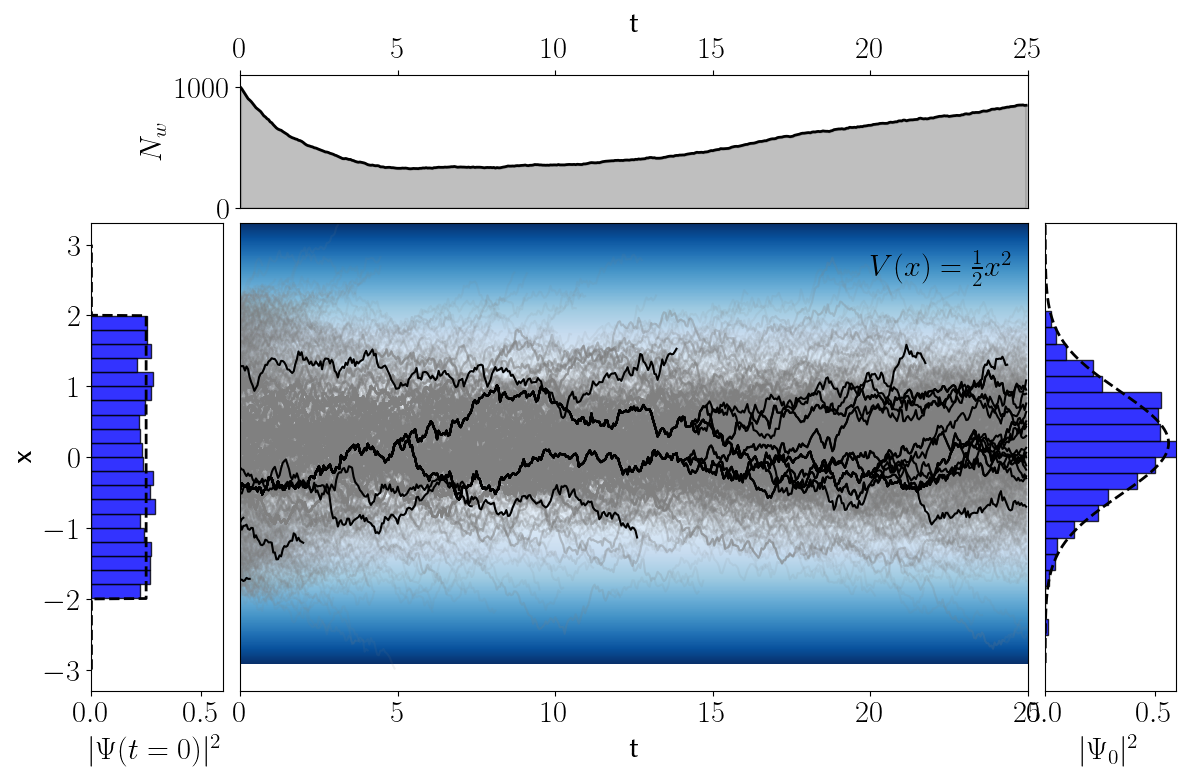
\includegraphics[width=\linewidth]{Chapter2/Figs/Raster/dmc.png}
	\caption[DMC simulation of harmonic oscillator]{\textbf{Diffusion Monte Carlo simulation of harmonic oscillator}, starting with $N_w=1000$ walkers, $\tau=0.05$, $E_c=0.25$ and uniformly sampling their initial positions from $(-2, 2)$ (\textbf{left}). The number of walkers at each step decreases rapidly before slowly increasing (\textbf{top}) the number of walkers is controlled by adjusting $E_c$. Walker paths, with a few highlighted in black to emphasise birth/death process (\textbf{middle}), diffuse into the approximate ground state of the HO $u_0(x) = \frac{1}{\pi^{\frac{1}{4}}}e^{-\frac{1}{2}x^2}$ (\textbf{right}).}
	\label{fig:dmc}
\end{figure}
Using a trial wave function $\Psi_T$ as a guiding function for importance sampling is an important improvement over vanilla DMC. This introduces a \emph{drift} into the diffusion process, which leads the walkers into regions of large values of $\Psi_T$ and greatly improves the statistical efficiency of the method. The guiding wave function is usually obtained by means of VMC. So far we have conveniently assumed that the wave function is positive everywhere in the domain, this not generally true, e.g. in fermionic systems, and poses a problem for PMC methods.

\subsubsection{The sign problem}
Projector Monte Carlo methods can only operate with positive distributions, and as such they fall apart when applied to fermionic or frustrated systems~\cite{gubernatis_kawashima_werner_2016}. A straightforward modification to the sampling scheme allows us to sample from a mixed-sign distribution. We sample from the distribution normally when it is positive, but sample from its absolute value and change the sign of the observable, when it is negative. The issue with this approach is that the population of configurations is split between positive and negative regions, the averages over both are comparable in size and cancel out, leading to a large statistical error compared to the observable. We refer to the accompanying exponential decrease~\cite{gubernatis_kawashima_werner_2016} in sampling efficiency with system size and temperature, \textbf{the sign problem}. Its general solution was shown to be NP-hard~\cite{troyer2005computational}, and as it is believed that P $\neq$ NP, this implies that no \emph{general} polynomial-time solutions exist. However, this does not mean that the problem cannot be avoided in special cases, the search for solutions is still an area of active research~\cite{hutcheon2020stochastic, assaraf2007fermion, alexandru2020complex}. In practice the sign problem is remedied by the \emph{fixed-node}~\cite{anderson1975random} or \emph{constrained-path}~\cite{zhang1997constrained} approximation. Fixed-node imposes a boundary condition into the projection such that the projected state shares the nodal surface with the trial wave function. The projected state is now only exact when the nodal surface is exact.

\section{Machine Learning and the quantum many-body problem}
With recent growing interest in Machine Learning there came a wave of research that applies ML methods to the natural sciences. As it pertains to the quantum many-body problem, most of the work is focused on exploiting the expressive nature of ML models, such as Restricted Boltzmann Machines (RBM)~\cite{carleo2017solving} or Deep Neural Networks~\cite{cai2018approximating} (DNN), to efficiently represent quantum states. These approaches fall into the VMC framework, and have been used for lattice models~\cite{carleo2017solving}, both fermionic~\cite{nomura2017restricted} and bosonic~\cite{saito2017solving}. Notably, special NN architectures have been used to achieve higher accuracies than coupled cluster calculations on a variety of atoms and small molecules~\cite{pfau2020ab, spencer2020better}. In lattice models Convolutional Neural Networks (CNN) have been shown to struggle to converge to nontrivial sign structures of frustrated systems, but modelling the phase and amplitude with separate networks helps in this regard~\cite{szabo2020neural}.

The expressiveness of RBM has also been analysed in depth~\cite{carleo2018constructing}, and contrasted to Tensor Network States~\cite{clark2018unifying}. Very recently an application of the NN ansatz in DMC with fixed-node approximation~\cite{wilson2021simulations} was used to improve earlier work results of the FermiNet~\cite{pfau2020ab}.

Alternatively to above approaches, which all operate in the Schr\" odinger picture, reinforcement learning has been used to solve the many-body problem in the path integral representation~\cite{barr2020quantum, gispen2020ground}. ML has also found place in mean field methods, perhaps most notably for learning the exchange and correlation functionals in DFT~\cite{dick2020machine}.

